% Template:     Informe LaTeX
% Documento:    Archivo de ejemplo
% Versión:      8.1.7 (24/07/2022)
% Codificación: UTF-8
%
% Autor: Pablo Pizarro R.
%        pablo@ppizarror.com
%
% Manual template: [https://latex.ppizarror.com/informe]
% Licencia MIT:    [https://opensource.org/licenses/MIT]

\section{Definición del Problema}

Desde la declaración de la pandemia Covid19 a nivel mundial, muchos han sido los esfuerzos de realizar acciones para entender y controlar el desarrollo de esta pandemia, sin embargo desde el campo de computación han surgido la necesidad de establecer herramientas que permitan análisis visual \scite{alsakran2020visual} que incorporen varios diseños visuales y análisis de las tendencias de propagación, con el objetivo de promover la comprensión de como se comportan los datos, ahora bien, a pesar que la pandemia a terminado, consideramos que sigue siendo una necesidad para el gobierno peruano y las instituciones llamadas a contribuir con herramientas que permitan el análisis y visualización de datos con otras enfermedades que azota al país como el caso del dengue, razón por la cual abordamos el presente trabajo.


\section{Descripción de la Base de Datos}


Covid19Mexico.csv \scite{salud} es una base de datos abiertos gestionado por la dirección general de epidemiología de la secretaría de salud de México, Conforme al Decreto publicado en el diario Oficial de la Federación el 20 de Febrero del 2015, que establece la regulación en materia de Datos Abiertos, la Dirección General de Epidemiología, con base en los ordenamientos aplicables en dicha materia, pone a disposición de la población en general, la información contenida en los Anuarios Estadísticos de Morbilidad 2015-2017, así como la información referente a los casos asociados a COVID-19 \scite{klein2023spatial} con el propósito de facilitar a todos los usuarios que la requieran, el acceso, uso, reutilización y redistribución de la misma.


\subsection{Definición de cada Atributo}
El \textit{dataset} fue obtenido del sitio web de datos abiertos del gobierno de los Estados Unidos Mexicanos \scite{Salud}, donde podemos encontrar toda la data
recolectada desde el 27 de noviembre de 2020 hasta el 16 de mayo de 2023; sin embargo, para este caso  tomaremos la base de datos que cuenta con 7294030 registros. Se escogió data, ya que permite ya que es mas manejable el análisis estadístico descriptivo y posibilitar su ejecución en computadores con características normales. En base al dataset recolectado se tienen los siguientes atributos:

\begin{enumerate}
	\item \textbf{FECHA\_ACTUALIZACION}: La base de datos se alimenta diariamente, esta variable permite identificar la fecha de la ultima actualizacion. AAAA-MM-DD
	\item \textbf{ID\_REGISTRO}: Número identificador del caso, TEXTO
	\item \textbf{ORIGEN}: La vigilancia centinela se realiza a través del sistema de unidades de salud monitoras de enfermedades respiratorias (USMER). Las USMER incluyen unidades médicas del primer, segundo o tercer nivel de atención y también participan como USMER las unidades de tercer nivel que por sus características contribuyen a ampliar el panorama de información epidemiológica, entre ellas las que cuenten con especialidad de neumología, infectología o pediatría. (Categorías en Catalógo Anexo). CATÁLOGO: ORIGEN
	\item \textbf{SECTOR}: Identifica el tipo de institución del Sistema Nacional de Salud que brindó la atención. CATÁLOGO: SECTOR
	\item \textbf{ENTIDAD\_UM}: Identifica la entidad donde se ubica la unidad medica que brindó la atención. CATALÓGO: ENTIDADES
	\item \textbf{SEXO}: Identifica al sexo del paciente. CATÁLOGO: SEXO
	\item \textbf{ENTIDAD\_NAC}: Identifica la entidad de nacimiento del paciente. CATALÓGO: ENTIDADES
	\item \textbf{ENTIDAD\_RES}: Identifica la entidad de residencia del paciente. CATALÓGO: ENTIDADES
	\item \textbf{MUNICIPIO\_RES}: Identifica el municipio de residencia del paciente. CATALÓGO: MUNICIPIOS
	\item \textbf{TIPO\_PACIENTE}: Identifica el tipo de atención que recibió el paciente en la unidad. Se denomina como ambulatorio si regresó a su casa o se denomina como hospitalizado si fue ingresado a hospitalización. CATÁLOGO: TIPO\_PACIENTE
	\item \textbf{FECHA\_INGRESO}: Identifica la fecha de ingreso del paciente a la unidad de atención. AAAA-MM-DD
	\item \textbf{FECHA\_SINTOMAS}: Idenitifica la fecha en que inició la sintomatología del paciente. AAAA-MM-DD
	\item \textbf{FECHA\_DEF}: Identifica la fecha en que el paciente falleció. AAAA-MM-DD
	\item \textbf{INTUBADO}: Identifica si el paciente requirió de intubación. CATÁLOGO: SI\_NO
	\item \textbf{NEUMONIA}: Identifica si al paciente se le diagnosticó con neumonía. CATÁLOGO: SI\_NO
	\item \textbf{EDAD}: Identifica la edad del paciente. NÚMERICA EN AÑOS
	\item \textbf{NACIONALIDAD}: Identifica si el paciente es mexicano o extranjero. CATÁLOGO: NACIONALIDAD
	\item \textbf{EMBARAZO}: Identifica si la paciente está embarazada. CATÁLOGO: SI\_NO
	\item \textbf{HABLA\_LENGUA\_INDIG}: Identifica si el paciente habla lengua índigena. CATÁLOGO: SI\_NO
	\item \textbf{INDIGENA}: Identifica si el paciente se autoidentifica como una persona indígena. CATÁLOGO: SI\_NO
	\item \textbf{DIABETES}: Identifica si el paciente tiene un diagnóstico de diabetes. CATÁLOGO: SI\_NO
	\item \textbf{EPOC}: Identifica si el paciente tiene un diagnóstico de EPOC. CATÁLOGO: SI\_NO
	\item \textbf{ASMA}: Identifica si el paciente tiene un diagnóstico de asma. CATÁLOGO: SI\_NO
	\item \textbf{INMUSUPR}: Identifica si el paciente presenta inmunosupresión. CATÁLOGO: SI\_NO
	\item \textbf{HIPERTENSION}: Identifica si el paciente tiene un diagnóstico de hipertensión. CATÁLOGO: SI\_NO
	\item \textbf{OTRA\_COM}: Identifica si el paciente tiene diagnóstico de otras enfermedades. CATÁLOGO: SI\_NO
	\item \textbf{CARDIOVASCULAR}: Identifica si el paciente tiene un diagnóstico de enfermedades cardiovasculares. CATÁLOGO: SI\_NO
	\item \textbf{OBESIDAD}: Identifica si el paciente tiene diagnóstico de obesidad. CATÁLOGO: SI\_NO
	\item \textbf{RENAL\_CRONICA}: Identifica si el paciente tiene diagnóstico de insuficiencia renal crónica. CATÁLOGO: SI\_NO
	\item \textbf{TABAQUISMO}: Identifica si el paciente tiene hábito de tabaquismo. CATÁLOGO: SI\_NO
	\item \textbf{OTRO\_CASO}: Identifica si el paciente tuvo contacto con algún otro caso diagnósticado con SARS CoV-2. CATÁLOGO: SI\_NO
	\item \textbf{TOMA\_MUESTRA\_LAB}: Identifica si al paciente se le tomó muestra de laboratorio. CATÁLOGO: SI\_NO
	\item \textbf{RESULTADO\_LAB}: Identifica el resultado del análisis de la muestra reportado por el  laboratorio de la Red Nacional de Laboratorios de Vigilancia Epidemiológica (INDRE, LESP y LAVE) y laboratorios privados avalados por el InDRE cuyos resultados son registrados en SISVER. (Catálogo de resultados diagnósticos anexo). CATÁLOGO: RESULTADO\_LAB
	\item \textbf{TOMA\_MUESTRA\_ANTIGENO}: Identifica si al paciente se le tomó muestra de antígeno para SARS-CoV-2. CATÁLOGO: SI\_NO
	\item \textbf{RESULTADO\_ANTIGENO}: Identifica el resultado del análisis de la muestra de antígeno tomada al paciente. CATÁLOGO: RESULTADO\_ANTIGENO
	\item \textbf{CLASIFICACION\_FINAL}: Identifica si el paciente es un caso de COVID\-19 según el catálogo ``CLASIFICACION\_FINAL''. CATÁLOGO: CLASIFICACION\_FINAL
	\item \textbf{MIGRANTE}: Identifica si el paciente es una persona migrante. CATÁLOGO: SI\_NO
	\item \textbf{PAIS\_NACIONALIDAD}: Identifica la nacionalidad del paciente. TEXTO, 99\=SE IGNORA
	\item \textbf{PAIS\_ORIGEN}: Identifica el país del que partió el paciente rumbo a México. TEXTO, 97\=NO APLICA
	\item \textbf{UCI}: Identifica si el paciente requirió ingresar a una Unidad de Cuidados Intensivos. CATÁLOGO: SI\_NO
\end{enumerate}

\clearpage

\subsection{Distribución de las Variables}
\subsubsection{Tipos de Datos de las columnas del \emph{dataset}}
En la tabla \ref{tabla:datatype} se puede apreciar los tipos de dato para cada columna del \emph{dataset}. Se puede apreciar que las fechas se detectan como \emph{object}, por lo cual será necesario hacer una transformación de dichos datos.

\begin{table}[h]
\resizebox{7.5cm}{!} {

\begin{tabular}{|l|l|l|}
\hline
\# & Variable                & T. de dato \\ \hline
1  & FECHA\_ACTUALIZACION    & object     \\ \hline
2  & ID\_REGISTRO            & object     \\ \hline
3  & ORIGEN                  & int64      \\ \hline
4  & SECTOR                  & int64      \\ \hline
5  & ENTIDAD\_UM             & int64      \\ \hline
6  & SEXO                    & int64      \\ \hline
7  & ENTIDAD\_NAC            & int64      \\ \hline
8  & ENTIDAD\_RES            & int64      \\ \hline
9  & MUNICIPIO\_RES          & int64      \\ \hline
10 & TIPO\_PACIENTE          & int64      \\ \hline
11 & FECHA\_INGRESO          & object     \\ \hline
12 & FECHA\_SINTOMAS         & object     \\ \hline
13 & FECHA\_DEF              & object     \\ \hline
14 & INTUBADO                & int64      \\ \hline
15 & NEUMONIA                & int64      \\ \hline
16 & EDAD                    & int64      \\ \hline
17 & NACIONALIDAD            & int64      \\ \hline
18 & EMBARAZO                & int64      \\ \hline
19 & HABLA\_LENGUA\_INDIG    & int64      \\ \hline
20 & INDIGENA                & int64      \\ \hline
21 & DIABETES                & int64      \\ \hline
22 & EPOC                    & int64      \\ \hline
23 & ASMA                    & int64      \\ \hline
24 & INMUSUPR                & int64      \\ \hline
25 & HIPERTENSION            & int64      \\ \hline
26 & OTRA\_COM               & int64      \\ \hline
27 & CARDIOVASCULAR          & int64      \\ \hline
28 & OBESIDAD                & int64      \\ \hline
29 & RENAL\_CRONICA          & int64      \\ \hline
30 & TABAQUISMO              & int64      \\ \hline
31 & OTRO\_CASO              & int64      \\ \hline
32 & TOMA\_MUESTRA\_LAB      & int64      \\ \hline
33 & RESULTADO\_LAB          & int64      \\ \hline
34 & TOMA\_MUESTRA\_ANTIGENO & int64      \\ \hline
35 & RESULTADO\_ANTIGENO     & int64      \\ \hline
36 & CLASIFICACION\_FINAL    & int64      \\ \hline
37 & MIGRANTE                & int64      \\ \hline
38 & PAIS\_NACIONALIDAD      & object     \\ \hline
39 & PAIS\_ORIGEN            & object     \\ \hline
40 & UCI                     & int64      \\ \hline
\end{tabular}
}
\caption{Tipos de datos del \emph{dataset}.}
\label{tabla:datatype}
\end{table}

\clearpage
\subsubsection{Valores no Nulos y Valores Nulos}
Si bien es cierto los datos mostrados en la tabla \ref{tabla:isnull} indican que la tabla no tiene valores nulos, al hacer una revisión del contenido
se encontró que muchos tienen valores 97, 98 y 99, que corresponden a "No aplica", "Se ignora", o "No especificado", respectivamente.

\begin{table}[h]
\resizebox{10cm}{!} {
\begin{tabular}{|l|l|c|c|}
\hline
\# & Variable & \multicolumn{1}{l|}{\# Valores Nulos} & \multicolumn{1}{l|}{\# Valores no Nulos} \\ \hline
1  & FECHA\_ACTUALIZACION    & 0 & 7294030 \\ \hline
2  & ID\_REGISTRO            & 0 & 7294030 \\ \hline
3  & ORIGEN                  & 0 & 7294030 \\ \hline
4  & SECTOR                  & 0 & 7294030 \\ \hline
5  & ENTIDAD\_UM             & 0 & 7294030 \\ \hline
6  & SEXO                    & 0 & 7294030 \\ \hline
7  & ENTIDAD\_NAC            & 0 & 7294030 \\ \hline
8  & ENTIDAD\_RES            & 0 & 7294030 \\ \hline
9  & MUNICIPIO\_RES          & 0 & 7294030 \\ \hline
10 & TIPO\_PACIENTE          & 0 & 7294030 \\ \hline
11 & FECHA\_INGRESO          & 0 & 7294030 \\ \hline
12 & FECHA\_SINTOMAS         & 0 & 7294030 \\ \hline
13 & FECHA\_DEF              & 0 & 7294030 \\ \hline
14 & INTUBADO                & 0 & 7294030 \\ \hline
15 & NEUMONIA                & 0 & 7294030 \\ \hline
16 & EDAD                    & 0 & 7294030 \\ \hline
17 & NACIONALIDAD            & 0 & 7294030 \\ \hline
18 & EMBARAZO                & 0 & 7294030 \\ \hline
19 & HABLA\_LENGUA\_INDIG    & 0 & 7294030 \\ \hline
20 & INDIGENA                & 0 & 7294030 \\ \hline
21 & DIABETES                & 0 & 7294030 \\ \hline
22 & EPOC                    & 0 & 7294030 \\ \hline
23 & ASMA                    & 0 & 7294030 \\ \hline
24 & INMUSUPR                & 0 & 7294030 \\ \hline
25 & HIPERTENSION            & 0 & 7294030 \\ \hline
26 & OTRA\_COM               & 0 & 7294030 \\ \hline
27 & CARDIOVASCULAR          & 0 & 7294030 \\ \hline
28 & OBESIDAD                & 0 & 7294030 \\ \hline
29 & RENAL\_CRONICA          & 0 & 7294030 \\ \hline
30 & TABAQUISMO              & 0 & 7294030 \\ \hline
31 & OTRO\_CASO              & 0 & 7294030 \\ \hline
32 & TOMA\_MUESTRA\_LAB      & 0 & 7294030 \\ \hline
33 & RESULTADO\_LAB          & 0 & 7294030 \\ \hline
34 & TOMA\_MUESTRA\_ANTIGENO & 0 & 7294030 \\ \hline
35 & RESULTADO\_ANTIGENO     & 0 & 7294030 \\ \hline
36 & CLASIFICACION\_FINAL    & 0 & 7294030 \\ \hline
37 & MIGRANTE                & 0 & 7294030 \\ \hline
38 & PAIS\_NACIONALIDAD      & 0 & 7294030 \\ \hline
39 & PAIS\_ORIGEN            & 0 & 7294030 \\ \hline
40 & UCI                     & 0 & 7294030 \\ \hline
\end{tabular}
}
\caption{Valores nulos y no nulos encontrados en el \emph{dataset}.}
\label{tabla:isnull}
\end{table}

\clearpage
\subsubsection{Valores únicos}

\begin{table}[h]
\resizebox{7cm}{!} {
\begin{tabular}{|l|c|}
\hline
FECHA\_ACTUALIZACION    & 1                        \\ \hline
ID\_REGISTRO            & 7294030                  \\ \hline
ORIGEN                  & 2                        \\ \hline
SECTOR                  & 14                       \\ \hline
ENTIDAD\_UM             & 32                       \\ \hline
SEXO                    & 2                        \\ \hline
ENTIDAD\_NAC            & 33                       \\ \hline
ENTIDAD\_RES            & 32                       \\ \hline
MUNICIPIO\_RES          & 550                      \\ \hline
TIPO\_PACIENTE          & 2                        \\ \hline
FECHA\_INGRESO          & 501                      \\ \hline
FECHA\_SINTOMAS         & 501                      \\ \hline
FECHA\_DEF              & 501                      \\ \hline
INTUBADO                & 4                        \\ \hline
NEUMONIA                & 3                        \\ \hline
EDAD                    & 131                      \\ \hline
NACIONALIDAD            & 2                        \\ \hline
EMBARAZO                & 5                        \\ \hline
HABLA\_LENGUA\_INDIG    & 3                        \\ \hline
INDIGENA                & 3                        \\ \hline
DIABETES                & 3                        \\ \hline
EPOC                    & 3                        \\ \hline
ASMA                    & 3                        \\ \hline
INMUSUPR                & 3                        \\ \hline
HIPERTENSION            & 3                        \\ \hline
OTRA\_COM               & 3                        \\ \hline
CARDIOVASCULAR          & 3                        \\ \hline
OBESIDAD                & 3                        \\ \hline
RENAL\_CRONICA          & 3                        \\ \hline
TABAQUISMO              & 3                        \\ \hline
OTRO\_CASO              & 3                        \\ \hline
TOMA\_MUESTRA\_LAB      & 2                        \\ \hline
RESULTADO\_LAB          & 5                        \\ \hline
TOMA\_MUESTRA\_ANTIGENO & \multicolumn{1}{l|}{2}   \\ \hline
RESULTADO\_ANTIGENO     & \multicolumn{1}{l|}{3}   \\ \hline
CLASIFICACION\_FINAL    & \multicolumn{1}{l|}{7}   \\ \hline
MIGRANTE                & \multicolumn{1}{l|}{3}   \\ \hline
PAIS\_NACIONALIDAD      & \multicolumn{1}{l|}{177} \\ \hline
PAIS\_ORIGEN            & \multicolumn{1}{l|}{113} \\ \hline
UCI                     & \multicolumn{1}{l|}{4}   \\ \hline
\end{tabular}
}
\caption{Cantidad de valores únicos.}
\label{tabla:autores}
\end{table}

\textbf{Valores únicos por columna}
\begin{lstlisting}[language=haskell, caption=Valores por columna, captionpos=b, label=lst:fiboHaskell]

FECHA_ACTUALIZACION
['2023-05-16']

ID_REGISTRO
['0741e4' '0ed066' '08c5f9' ... 'm19f073' 'm1e288e' 'm1029da']

ORIGEN
[2 1]

SECTOR
[ 6 12  3  9 10 11  8  7  1  4  5 13  2 99]

ENTIDAD_UM
[ 9 16 15 12 22 18 20 14 23 25  3 10  7 17 24  5  1 21 28 26 27 19  4  2
 32 31  8 13 11 30  6 29]

SEXO
[2 1]

ENTIDAD_NAC
[ 9 16 12 18 20 32  8 25 14 10  7 27  6 13 15 17 22 24  5 21 28 26 19  2
 31  1  3 11 29 30 99  4 23]

ENTIDAD_RES
[ 9 16 15 12 22 18 20 14 23 25  3 10  7 17 24  5  1 21 28 26 27 19  4  2
 32 31  8 13 11 30  6 29]

MUNICIPIO_RES
[ 16  41  60   2  14  29  15   7  67  71   6   8   1  12  10   3   5  59
 ...
 220 501 532 484 276 481 299 556 433 506]

TIPO_PACIENTE
[2 1]

FECHA_INGRESO
['2022-02-20' '2023-03-09' '2022-01-11' '2022-08-07' '2022-05-22'
 ...
 '2023-05-16']

FECHA_SINTOMAS
['2022-02-13' '2023-03-06' '2022-01-09' '2022-02-20' '2022-08-07'
 ...
 '2023-05-16']

FECHA_DEF
['2022-02-21' '9999-99-99' '2022-09-10' '2022-01-12' '2022-01-01'
 ...
 '2023-05-14']

INTUBADO
[ 2 97 99  1]

NEUMONIA
[ 1  2 99]

EDAD
[ 54  28  63   3  58  50  56  52  24  57  55  23  81  33  43  39  41  35
  49  27  34  51  68  59  62  40  26  36  44  73  37   0  46  42  48  14
  31  67  21  32  61  69  47  70  82  76  25  38   5  29  53  84  75  30
  12  20  65   9  66  64  13  71   2  72  60  86  19  18  83  11   1  16
  92  17   4  22  79  45   6  74  15  96  88  77   8  10  85   7  87  91
  99  78  80  90  95  89  94  93  97  98 105 103 100 107 106 108 102 109
 101 119 122 110 113 114 120 115 104 112 111 116 117 121 118 123 135 130
 137 266 164 141 154]

NACIONALIDAD
[1 2]

EMBARAZO
[97  2 98  1 99]

HABLA_LENGUA_INDIG
[ 2 99  1]

INDIGENA
[ 2 99  1]

DIABETES
[ 2  1 98]

EPOC
[ 2 98  1]

ASMA
[ 2  1 98]

INMUSUPR
[ 2 98  1]

HIPERTENSION
[ 1  2 98]

OTRA_COM
[ 2 98  1]

CARDIOVASCULAR
[ 2 98  1]

OBESIDAD
[ 2 98  1]

RENAL_CRONICA
[ 1  2 98]

TABAQUISMO
[ 2  1 98]

OTRO_CASO
[ 2  1 99]

TOMA_MUESTRA_LAB
[1 2]

RESULTADO_LAB
[ 4 97  1  2  3]

TOMA_MUESTRA_ANTIGENO
[2 1]

RESULTADO_ANTIGENO
[97  2  1]

CLASIFICACION_FINAL
[2 7 5 3 6 1 4]

MIGRANTE
[99  1  2]

PAIS_NACIONALIDAD
['México' 'Estados Unidos de América' 'Cuba' 'Venezuela' 'El Salvador'
 'Taiwán' 'Argentina' 'Guatemala' 'España' 'Suecia' 'Holanda' 'Haití'
 ...
 'Burundi' 'Surinam' 'Moldavia' '99' 'República de Namibia']

PAIS_ORIGEN
['97' 'Estados Unidos de América' 'Cuba' 'Venezuela' 'Suecia' 'Otro'
 'Emiratos Arabes Unidos' 'Canadá' 'Francia' 'Haití'
 ...
 'Georgia' 'Reino Hachemita de Jordania' 'Surinam' 'Níger']

UCI
[ 2 97 99  1]


\end{lstlisting}

\clearpage

\subsubsection{Medidas de dispersión}
\begin{table}[h]
\resizebox{15cm}{!} {

\begin{tabular}{|l|c|c|c|c|c|c|c|c|}
\hline
\multicolumn{1}{|c|}{\textbf{index}} & \textbf{count} & \textbf{mean} & \textbf{std} & \textbf{min} & \textbf{25\%} & \textbf{50\%} & \textbf{75\%} & \textbf{max} \\ \hline
ORIGEN                  & 7294030 & 1.763377858 & 0.425008386 & 1 & 2  & 2  & 2  & 2   \\ \hline
SECTOR                  & 7294030 & 7.757825098 & 3.953231221 & 1 & 4  & 8  & 12 & 99  \\ \hline
ENTIDAD\_UM             & 7294030 & 14.54213048 & 7.903912713 & 1 & 9  & 11 & 21 & 32  \\ \hline
SEXO                    & 7294030 & 1.430898694 & 0.495202023 & 1 & 1  & 1  & 2  & 2   \\ \hline
ENTIDAD\_NAC            & 7294030 & 15.62352335 & 10.63514472 & 1 & 9  & 14 & 21 & 99  \\ \hline
ENTIDAD\_RES            & 7294030 & 14.73218934 & 7.852394862 & 1 & 9  & 13 & 21 & 32  \\ \hline
MUNICIPIO\_RES          & 7294030 & 37.77122003 & 90.13500533 & 1 & 7  & 16 & 39 & 999 \\ \hline
TIPO\_PACIENTE          & 7294030 & 1.04401586  & 0.205130372 & 1 & 1  & 1  & 1  & 2   \\ \hline
INTUBADO                & 7294030 & 92.8346918  & 19.45689118 & 1 & 97 & 97 & 97 & 99  \\ \hline
NEUMONIA                & 7294030 & 2.92867674  & 9.538137877 & 1 & 2  & 2  & 2  & 99  \\ \hline
EDAD                    & 7294030 & 37.46539279 & 17.70981582 & 0 & 25 & 36 & 49 & 266 \\ \hline
NACIONALIDAD            & 7294030 & 1.007355193 & 0.085446447 & 1 & 1  & 1  & 1  & 2   \\ \hline
EMBARAZO                & 7294030 & 43.50648859 & 47.14052115 & 1 & 2  & 2  & 97 & 99  \\ \hline
HABLA\_LENGUA\_INDIG    & 7294030 & 7.827968352 & 23.06138331 & 1 & 2  & 2  & 2  & 99  \\ \hline
INDIGENA                & 7294030 & 7.696031001 & 22.81939526 & 1 & 2  & 2  & 2  & 99  \\ \hline
DIABETES                & 7294030 & 2.288756696 & 5.797524763 & 1 & 2  & 2  & 2  & 98  \\ \hline
EPOC                    & 7294030 & 2.335288997 & 5.713323054 & 1 & 2  & 2  & 2  & 98  \\ \hline
ASMA                    & 7294030 & 2.3198694   & 5.696650467 & 1 & 2  & 2  & 2  & 98  \\ \hline
INMUSUPR                & 7294030 & 2.333863721 & 5.698540759 & 1 & 2  & 2  & 2  & 98  \\ \hline
HIPERTENSION            & 7294030 & 2.252608777 & 5.710399184 & 1 & 2  & 2  & 2  & 98  \\ \hline
OTRA\_COM               & 7294030 & 3.409708488 & 11.59610277 & 1 & 2  & 2  & 2  & 98  \\ \hline
CARDIOVASCULAR          & 7294030 & 2.331187423 & 5.702850698 & 1 & 2  & 2  & 2  & 98  \\ \hline
OBESIDAD                & 7294030 & 2.265451198 & 5.592334287 & 1 & 2  & 2  & 2  & 98  \\ \hline
RENAL\_CRONICA          & 7294030 & 2.331622985 & 5.698980204 & 1 & 2  & 2  & 2  & 98  \\ \hline
TABAQUISMO              & 7294030 & 2.300511514 & 5.728448784 & 1 & 2  & 2  & 2  & 98  \\ \hline
OTRO\_CASO              & 7294030 & 3.839758405 & 14.06565462 & 1 & 2  & 2  & 2  & 99  \\ \hline
TOMA\_MUESTRA\_LAB      & 7294030 & 1.844880813 & 0.36201829  & 1 & 2  & 2  & 2  & 2   \\ \hline
RESULTADO\_LAB          & 7294030 & 82.22869141 & 34.47462806 & 1 & 97 & 97 & 97 & 97  \\ \hline
TOMA\_MUESTRA\_ANTIGENO & 7294030 & 1.12586019  & 0.331691751 & 1 & 1  & 1  & 1  & 2   \\ \hline
RESULTADO\_ANTIGENO     & 7294030 & 13.52942228 & 31.67630136 & 1 & 1  & 2  & 2  & 97  \\ \hline
CLASIFICACION\_FINAL    & 7294030 & 5.014349955 & 2.009168658 & 1 & 3  & 6  & 7  & 7   \\ \hline
MIGRANTE                & 7294030 & 98.34537012 & 7.952658269 & 1 & 99 & 99 & 99 & 99  \\ \hline
UCI                     & 7294030 & 92.83490498 & 19.4559239  & 1 & 97 & 97 & 97 & 99  \\ \hline
\end{tabular}
}
\caption{Medidas de dispersión}
\label{tabla:autores}
\end{table}


\clearpage
\subsubsection{Correlación de variables}


\begin{table}[h]
\resizebox{7cm}{!} {

\begin{tabular}{|l|c|}
\hline
\multicolumn{1}{|c|}{\textbf{UCI}} & \textbf{1.000000} \\ \hline
INTUBADO                           & 0.999998          \\ \hline
NEUMONIA                           & 0.274011          \\ \hline
TOMA\_MUESTRA\_LAB                 & 0.223266          \\ \hline
RESULTADO\_LAB                     & 0.222660          \\ \hline
SECTOR                             & 0.161362          \\ \hline
ORIGEN                             & 0.127002          \\ \hline
HABLA\_LENGUA\_INDIG               & 0.052569          \\ \hline
INDIGENA                           & 0.051768          \\ \hline
INMUSUPR                           & 0.019560          \\ \hline
CARDIOVASCULAR                     & 0.019523          \\ \hline
ASMA                               & 0.019085          \\ \hline
OTRA\_COM                          & 0.019068          \\ \hline
TABAQUISMO                         & 0.018565          \\ \hline
DIABETES                           & 0.018240          \\ \hline
HIPERTENSION                       & 0.017668          \\ \hline
RENAL\_CRONICA                     & 0.015577          \\ \hline
OBESIDAD                           & 0.013859          \\ \hline
EPOC                               & 0.009055          \\ \hline
NACIONALIDAD                       & 0.008632          \\ \hline
MIGRANTE                           & -0.008154         \\ \hline
OTRO\_CASO                         & -0.024677         \\ \hline
EMBARAZO                           & -0.033323         \\ \hline
SEXO                               & -0.035863         \\ \hline
ENTIDAD\_NAC                       & -0.048609         \\ \hline
CLASIFICACION\_FINAL               & -0.065511         \\ \hline
ENTIDAD\_UM                        & -0.082240         \\ \hline
ENTIDAD\_RES                       & -0.082378         \\ \hline
EDAD                               & -0.083412         \\ \hline
TOMA\_MUESTRA\_ANTIGENO            & -0.123367         \\ \hline
RESULTADO\_ANTIGENO                & -0.124028         \\ \hline
MUNICIPIO\_RES                     & -0.135068         \\ \hline
TIPO\_PACIENTE                     & -0.997226         \\ \hline
\end{tabular}
}
\caption{Correlación de variables}
\label{tabla:autores}
\end{table}


\clearpage
\begin{figure}[h]
	\centering
	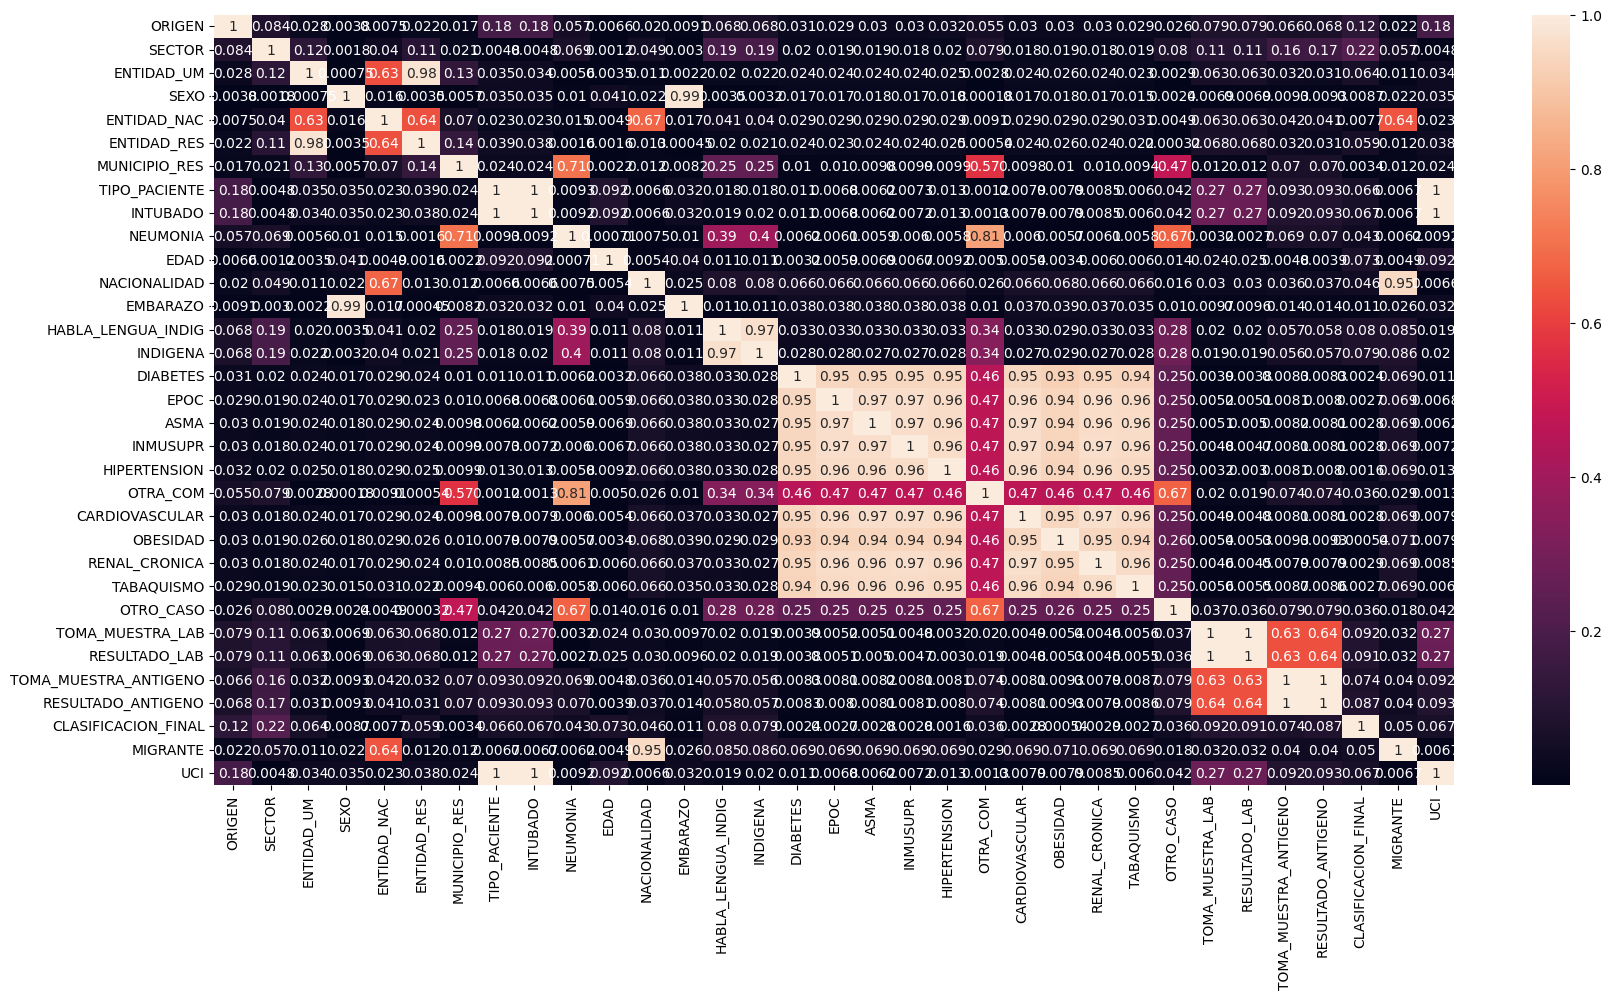
\includegraphics[scale=.4] {img/a-correlacion}
	\caption{Matriz de correlación}
	\label{fig:0}	
\end{figure}

% ------------------------------------------------------------------------------
% REFERENCIAS, revisar configuración \stylecitereferences
% ------------------------------------------------------------------------------
\clearpage
\bibliography{library} 